\section{Experiments}

\subsection{Benchmarks}

\subsubsection{Arcade Learning Environment}

\editnote{TODO: Include paragraph about partial observability of ALE.}

The Arcade Learning Environment (ALE) has became a platform for evaluating artificial intelligence agents. Originally proposed by Bellemare et. al. \cite{Code.ALE}, the ALE makes available dozens of Atari 2600 games for an agent training and evaluation. The agent is expected to do well in as many games as possible without game-specific information, generally perceiving the world through a video stream. Atari 2600 games are excellent environments for evaluating AI agents for three main reasons: they are varied enough to provide multiple different tasks, requiring general competence, they are interesting and challenging for humans and they are free of experimenter’s bias, having been developed by an independent party.

In the context of the ALE, a discrete action is a number in range from 0 to 17 inclusive which encodes the composition of a joystick direction and an optional button press. The agent observes a reward signal, which is typically the change in the player’s score (the difference in score between the previous time step and the current time step), and an observation $o_t \in O$ of the environment. This observation can take form of a single 210 × 160 image and/or the current 1024-bit RAM state. Because a single image typically does not satisfy the Markov property the ALE is formalised as POMDP. Observations and the environment state are distinguished, with the RAM data being the real state of the emulator. A frame (as a unit of time) corresponds to 1/60th of a second, the time interval between two consecutive images rendered to the television screen. The ALE is deterministic, which means that given a particular emulator state $s$ and a action $a$ there is a unique next state $s'$, that is, $P^a_{ss'} = p(s' | s, a) = 1$.

Agents interact with the ALE in an episodic fashion. An episode begins by resetting the environment to its initial configuration, $s_0$, and ends at a given endpoint depending on a game. The primary measure of an agent’s performance is the score achieved during an episode, namely the undiscounted sum of rewards for that episode. While this performance measure is quite natural, it is important to realize that score is not necessarily an indicator of AI progress. In some games, agents can exploit the game's mechanics to maximize sum of rewards, but not complete the game's goal in human's understanding. \cite{Study.FaultyReward}

Preprocessing include frame skipping \cite{Study.FrameSkipping} which restricts the agent’s decision points by repeating a selected action for 4 consecutive frames. Frame skipping results in a simpler reinforcement learning problem and speeds up execution.
\editnote{TODO: Describe other preprocessing techniques used here.}

This work uses ALE through OpenAI Gym API \cite{Code.OpenAIGym}, specifically two games are used as benchmarks: Boxing and Freeway.

Boxing is a video game based on the sport of boxing. Boxing shows a top-down view of two boxers, one white and one black. When close enough, a boxer can hit his opponent with a punch. This causes his opponent to reel back slightly and the boxer scores a point, a reward of 1. In the other situation, when the boxer gets hit, he gets a negative reward of -1. There are no knockdowns or rounds. A match is completed either when one player lands 100 punches (a 'knockout') or two minutes have elapsed. In the case of a decision, the player with the most landed punches is the winner. Ties are possible. 
While the gameplay is simple, there are subtleties, such as getting an opponent on the 'ropes' and 'juggling' him back and forth between alternate punches. 

\begin{figure}[H]
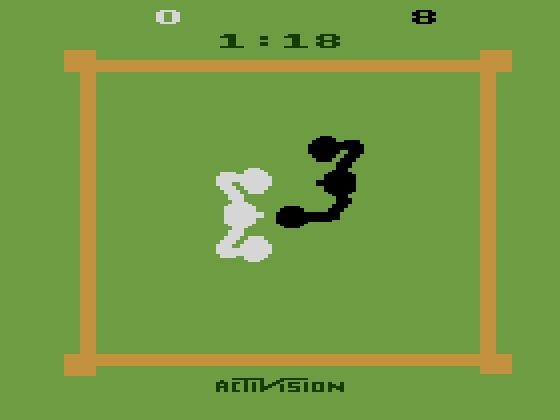
\includegraphics[width=0.5\textwidth,keepaspectratio]{figures/Boxing.jpg}
\caption[Boxing]{Example of Boxing level}
\label{Fig.Boxing}
\end{figure}

In Freeway an agent controls a chicken who can be made to run across a ten lane highway filled with traffic in an effort to "get to the other side." Every time a chicken gets across a reward of 1 is earned by the agent. If hit by a car, then a chicken is forced back slightly. The goal is to score as much points as possible in the two minutes. The chicken is only allowed to move up or down. 
The major challenge in this environment are sparse rewards. The agent scores only when successfully crosses the highway, which is not a trivial task.

\begin{figure}[H]
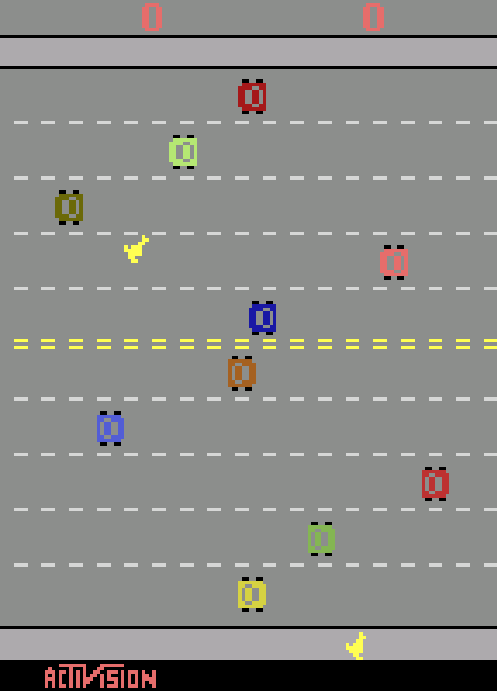
\includegraphics[width=0.5\textwidth,keepaspectratio]{figures/Freeway.png}
\caption[Freeway]{Example of Freeway level}
\label{Fig.Freeway}
\end{figure}

\editnote{TODO: Add more games if needed.}

\subsubsection{Sokoban}

\editnote{TODO: Include paragraph about fully observability of Sokoban state.}

Sokoban is a classic planning problem. It is a challenging one-player puzzle game in which the goal is to navigate a grid world maze and push boxes onto target tiles. A Sokoban puzzle is considered solved when all boxes are positioned on top of target locations. The player can move in all 4 cardinal directions and only push boxes into an empty space (as opposed to pulling). For this reason many moves are irreversible and mistakes can render the puzzle unsolvable. A human player is thus forced to plan moves ahead of time. Artificial agents should similarly benefit from a learned model and simulation.

Despite its simple rule set, Sokoban is an incredibly complex game for which no general solver exists. It can be shown that Sokoban is NP-Hard and PSPACE-complete \cite{Benchmark.Sokoban}. Sokoban has an enormous state space that makes it inassailable to exhaustive search methods. An efficient automated solver for Sokoban must have strong heuristics, just as humans utilize their strong intuition, so that it is not overwhelmed by the number of possible game states.

The implementation of Sokoban\cite{Code.Sokoban} used for those experiments procedurally generates a new level each episode. This means an agent cannot memorize specific puzzles. Together with the planning aspect, this makes for a very challenging environment. While the underlying game logic operates in a 10 × 10 grid world, agents were trained directly on RGB sprite graphics. Fig.~\ref{Fig.Sokoban} shows an example of Sokoban level with 4 boxes.

\editnote{TODO: Go into deeper details about e.g. how rewards are obtained etc.}

\begin{figure}[H]
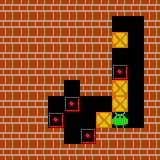
\includegraphics[]{figures/Sokoban.png}
\caption[Sokoban]{Example of Sokoban level}
\label{Fig.Sokoban}
\end{figure}

\subsection{Hardware}

\editnote{TODO: Add HW specification.}

\subsection{World Models for Sokoban}

This section focuses on a problem of model learning in Sokoban that is used to solve the environment. The goal was to train a model to generate sharp and accurate open loop predictions of observations and obtain high score using it. In theory, how probable are sequences of ground truth observations is measured using log probability. In practice, though, it is far more useful to compare those generated sequences of future observations with ground truth sequences with an eye of the researcher. What the researcher looks for are sharp generated images which accurately resemble frames from the game. Moreover, the sequence needs to simulate subsequent actions properly, otherwise it is told that the sequence is noisy or does not model actions issued well.

To generate an open loop prediction 60 consecutive frames and actions on average are fed into the model to initialize its hidden state first. Then, the model is ready to generate an open loop future prediction with its memory module by feeding it with subsequent actions and its own predictions as a contemporary state at following time steps. Reader should notice that what gets generated are not frames, but latent state's vectors. Those latent states can then be decoded into images for inspection.

\subsubsection{Train the unchanged World Models implementation in the Sokoban environment}

In this experiment, the original World Models was trained in the Sokoban environment. No modification to the original method described in the related work chapter was made, beyond addition of the deterministic variant of memory module described in the previous chapter.

The vision model successfully learned to encode high dimensional observations into low dimensional latent states. Fig.~\ref{Fig.WM_Sokoban_vision} shows original observations (first and third columns) side by side with reconstructed observations from their encodings (second and fourth columns). These are zero step predictions, no future is predicted only encoding to latent space and decoding to image space again is done.

\begin{figure}[H]
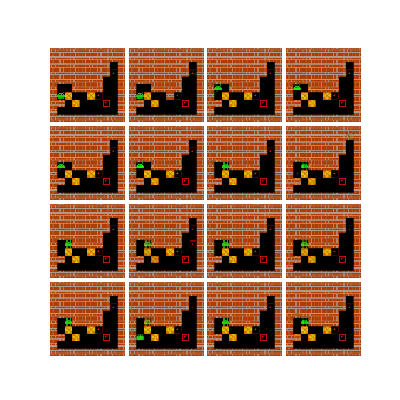
\includegraphics[width=1\textwidth,keepaspectratio]{figures/Sokoban_vision.png}
\caption[Qualitative result of the World Models vision model training in Sokoban]{Qualitative result of the vision model training in Sokoban. First and third columns include original observations. Second and fourth columns include reconstructions. Each reconstruction was obtained by first encoding the original observation and then decoding it, using VAE encoder and decoder respectively.}
\label{Fig.WM_Sokoban_vision}
\end{figure}

The stochastic and deterministic memory models were not able to learn Sokoban’s dynamics. Fig.~\ref{Fig.WM_Sokoban_memory} shows that the stochastic model very often can not determine the agents position. The agent disappears and blocks change their types. The eighth row shows that pushing mechanics are not modeled, the agent passes through boxes. The deterministic model does not do better.
The controller model failed to learn how to solve any level, it behaved comparably to a random play. We suspect that VAE is unable to generate usable abstract Sokoban representation and the shallow memory and controller models can not grasp complex dynamics of Sokoban using this poor representation. This idea is further developed in the next experiment.

\begin{figure}[H]
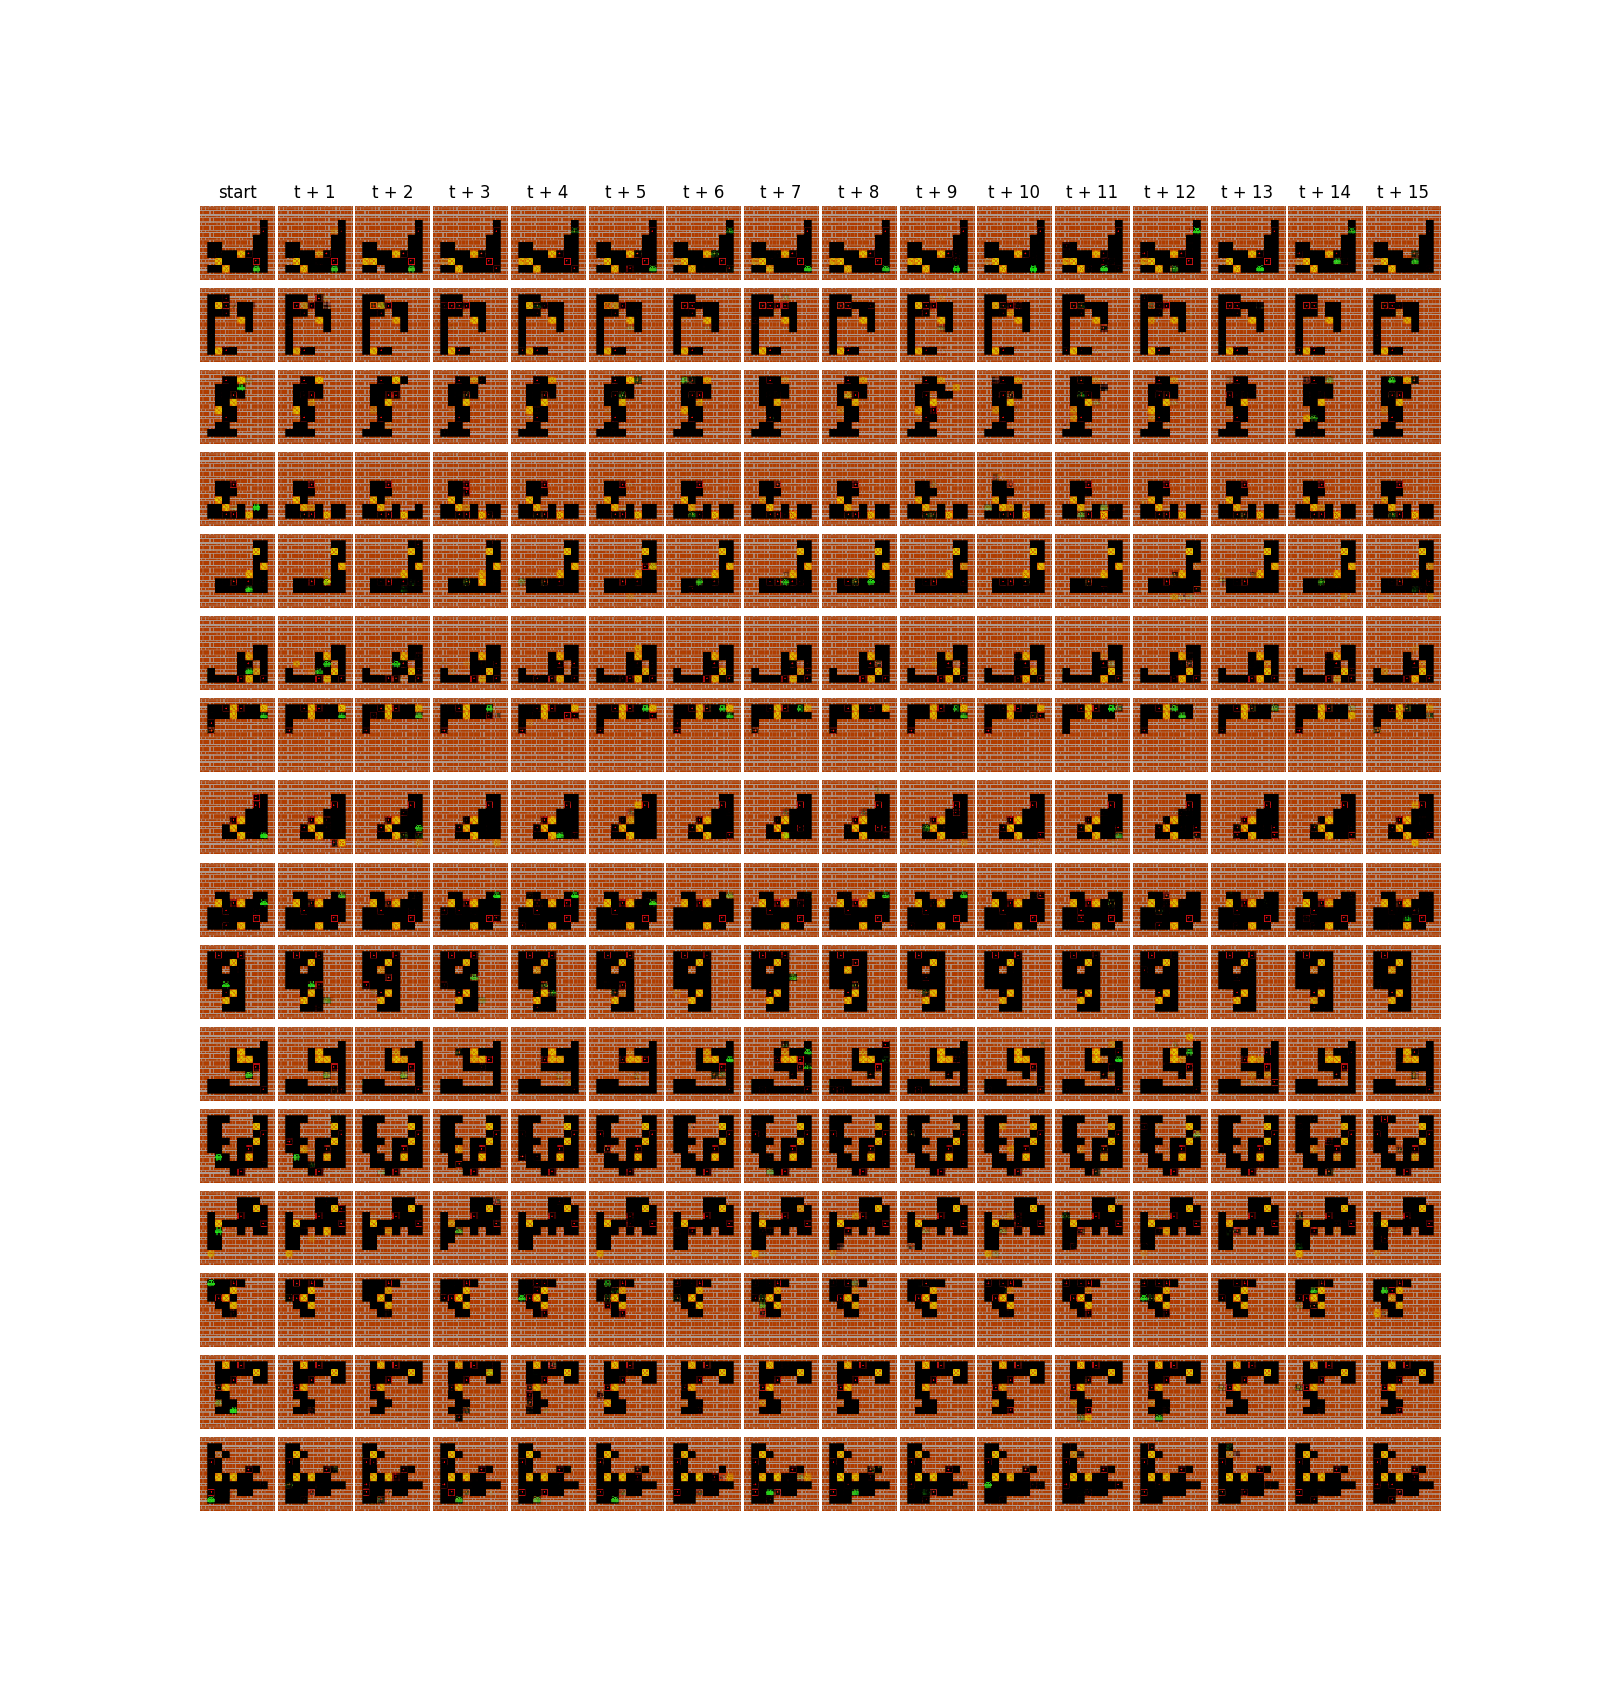
\includegraphics[width=1\textwidth,keepaspectratio]{figures/Sokoban_memory.png}
\caption[Qualitative result of the World Models memory model training in Sokoban]{Qualitative result of the memory model training in Sokoban. Each row depicts the memory model rollout in one episode. The first column include original observations from the evaluation dataset from which the rollouts start. The RNN's hidden state was initialized on preceding transitions in each episode. Each subsequent reconstruction was obtained by first predicting the next latent state by the memory model and then decoding it using the VAE decoder.}
\label{Fig.WM_Sokoban_memory}
\end{figure}

\subsubsection{Train World Models in Sokoban environment on 10x10 grid world states}

The latent state vector size is set to 64. This means that in theory this vector can accommodate full information about an observation. As noted before, Sokoban underlying game logic operates in a 10 × 10 grid world, where far edges of a level are always walls. This means that the level is described by 64 block types organized in an 8 x 8 grid. In this experiment, this domain knowledge is exploited and the agent uses those 64 block types as an input vector to the memory module, bypassing the vision model. It is worth noting, that the vision model should learn this representation as it is the optimal encoding when the objective is to compress a pixel image into a 64-dimensional vector and then reconstruct the original observation from it. However, despite use of the optimal encoding, the results have not been improved.

The proposed input format is optimal encoding if one wants to compress a pixel image and then reconstruct it. However, it is really poor representation of a current state of the environment if one wants to use linear combination of those features (block types in each position) to infer optimal next action and this is exactly what the controller model is tying to do. Modeling a value function could have more sense e.g. the value function could learn that a box on a target position yields higher value, but even it would have a hard time modeling more complex relations between entities in the environment. More useful for the controller would be e.g. representation that includes information about distance between the box and each target position. Nevertheless, this could be not enough too. The box on the target position would get discounted for not being on some other target positions. Hence, there is need for feature saying “the box X placed on the target position Y”. In the end, the linear combination of the proposed latent features can not model useful policy.

On the other hand, this representation includes, not well represented, but perfect information about an environment state. The memory model creates its own environment representation encoded in its hidden state and then uses this representation to predict the next latent state. This memory's hidden state is also utilized by the controller. Still, it does not seem to encode useful enough information for the two, memory and controller, to do well on their tasks. One way to improve the hidden state representation is explored in the next experiment.

\subsubsection{Train World Model in Sokoban with auxiliary tasks}

Auxiliary tasks\cite{Algo.AuxiliaryTasks} have proved to help create more informative representation of an environment. In this experiment, reward and value prediction tasks are added to the memory model. In short, two additional linear models are added on top of the RNN to predict the next reward in the environment and model a value function. In theory, it should help form a more informative hidden state of the memory model. Consequently, it should help learn Sokoban’s dynamics, but also generate representation on a higher level of abstraction that could prove useful for the controller. Moreover, a reward prediction will be needed in further work on planning with learned model.

For all that, the memory model have not been able to learn to predict the rewards and values. Also, there was no improvement in memory's and controller’s performance. It is suspected, that the main cause of this failure are sparse rewards in the training dataset. A random agent used to generate the dataset does not receive many positive rewards. Effectively, most of the episodes do not have any positive reward. Hence, the memory model soon overfit on more or less constant reward and value. 
This yields insight that the data generation procedure does not cover state-space well. Iterative approach to gathering data, from a better and better agent, could solve this problem.

It is not without significance that Sokoban has enormous state-space. Because each episode, or level, is randomly generated it is much different from the others - it is nearly impossible for an agent to see a similar state in a different episode. Hence, Sokoban requires strong generalization capability from the memory module. Simple RNN can lack capacity to create good representation and in turn achieve good prediction performance. For instance I2A\cite{Algo.I2A} uses deep neural network architecture to handle Sokoban complexity. A more flexible memory model with larger capacity could manage this complexity and need for generalization. The two insights are explored in the PlaNet experiments, which have larger model and uses iterative training procedure. However before that, World Models are tested in an easier environment, Boxing from Atari.

\subsection{World Models for Atari}

In two experiments below ideas from previous section were put into the test. Firstly, the original World Models is trained for the Boxing environment, which has dense rewards and data collection using a random agent cover most of the state-space. Then, World Models is coupled with AlphaZero planner and both are trained jointly.

\subsubsection{Train unchanged World Models in the Boxing environment}

In this experiment, the original World Models was trained in the Boxing environment. No modification to the original method described in the related work chapter was made. In this experiment discrete memory was not tested as original stochastic one did well.

The vision model successfully learned to encode high dimensional observations into low dimensional latent states. Fig.~\ref{Fig.WM_Boxing_vision} shows original observations (first and third columns) side by side with reconstructed observations from their encodings (second and fourth columns). These are zero step predictions, no future is predicted only encoding to latent space and decoding to image space again is done.

\begin{figure}[H]
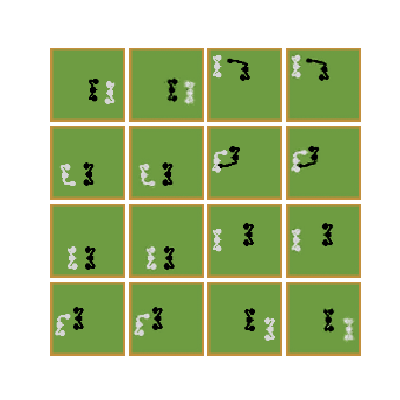
\includegraphics[width=1\textwidth,keepaspectratio]{figures/Boxing_vision.png}
\caption[Qualitative result of the World Models vision model training in Boxing]{Qualitative result of the vision model training in Boxing. First and third columns include original observations. Second and fourth columns include reconstructions. Each reconstruction was obtained by first encoding the original observation and then decoding it, using VAE encoder and decoder respectively.}
\label{Fig.WM_Boxing_vision}
\end{figure}

The stochastic memory models was able to learn Boxing’s dynamics. Fig.~\ref{Fig.WM_Boxing_memory} shows that the stochastic model generates very sharp and accurate predictions that model agents movement and punches really well. The agents does not disappear like in Sokoban and actions are smooth.
The controller model successfully learned how to solve the game scoring above 18 points on average across 5 runs. We suspect that World Models with latent state of size 16 was forced to encode two characters positions and hands states which are useful high-level features when deciding on the next action. It is worth pointing out here that similar experiment with such a small latent space did not yield improvement in Sokoban.

\begin{figure}[H]
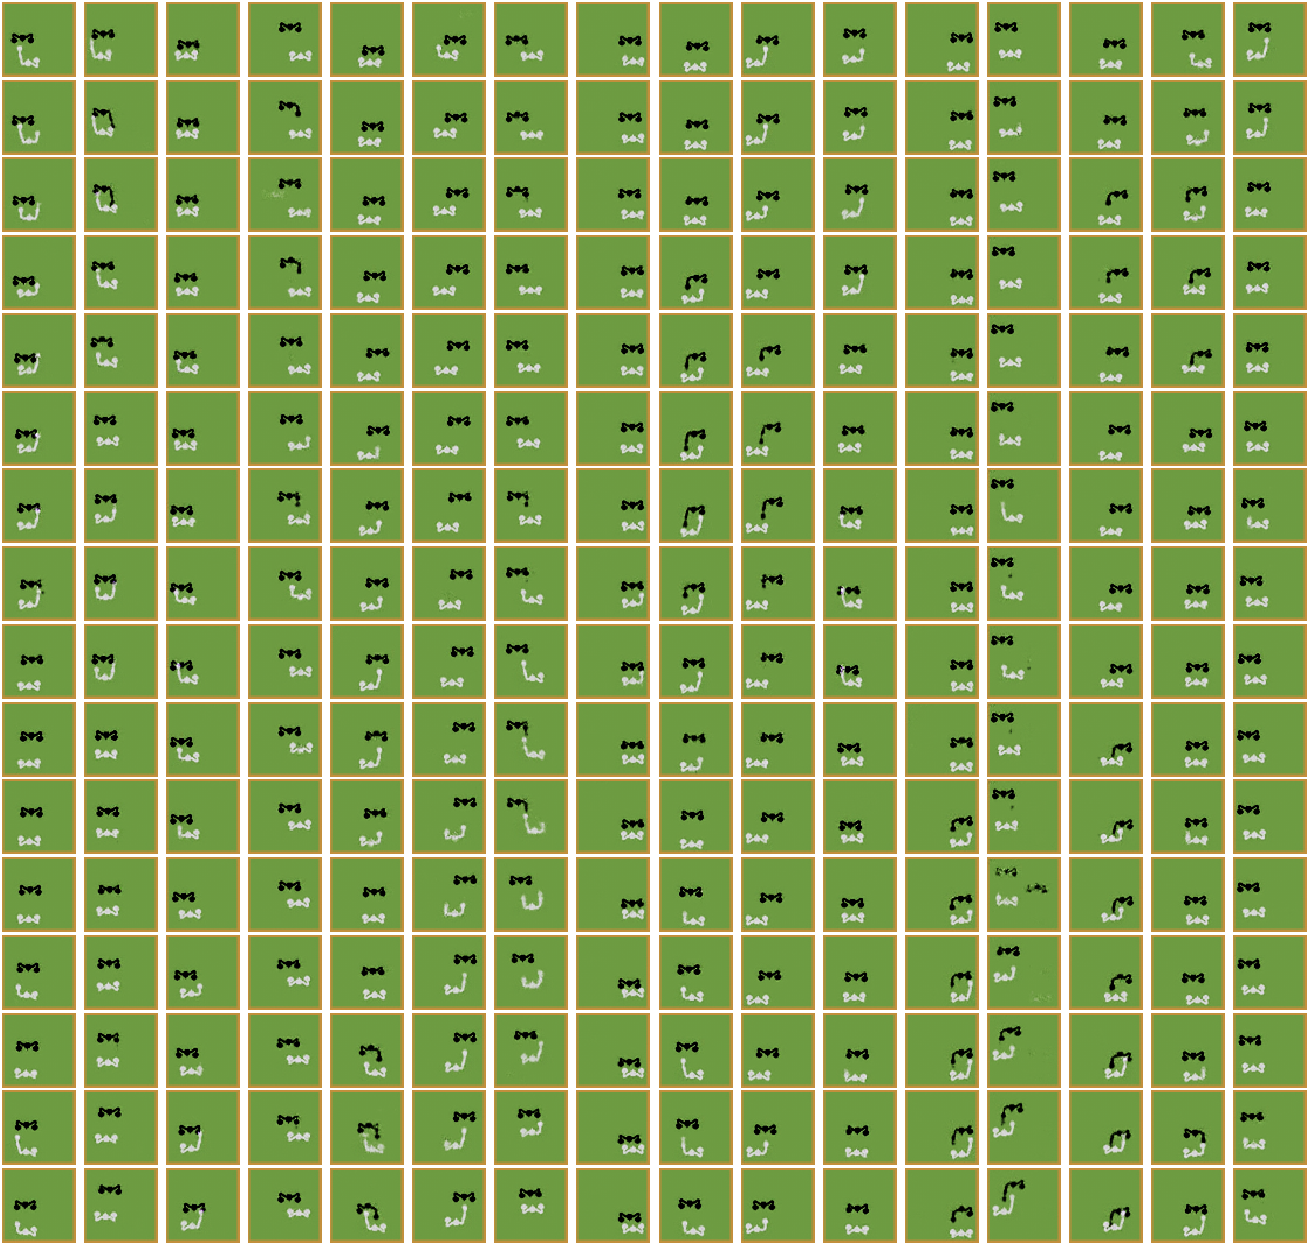
\includegraphics[width=1\textwidth,keepaspectratio]{figures/Boxing_memory.png}
\caption[Qualitative result of the World Models memory model training in Boxing]{Qualitative result of the memory model training in Boxing. Each row depicts the memory model rollout in one episode. The first column include original observations from the evaluation dataset from which the rollouts start. The RNN's hidden state was initialized on preceding transitions in each episode. Each subsequent reconstruction was obtained by first predicting the next latent state by the memory model and then decoding it using the VAE decoder.}
\label{Fig.WM_Boxing_memory}
\end{figure}

\subsubsection{Train World Models with AlphaZero planner in the Boxing environment}

Despite getting really accurate future predictions in the previous experiment and hyper-parameter tuning of this architecture the AlphaZero planner training was unstable. It did not train to properly plan in latent space and play the game. Decision was to abandon this solution and move to PlaNet which shown that, in deed, it is possible to plan in continuous control tasks.

\subsection{PlaNet for Sokoban}

\subsubsection{Train unchanged PlaNet in the Sokoban environment}

PlaNet did not capture Sokoban dynamics too. In the figure below (Fig.~\ref{Fig.PlaNet_Sokoban_openloop}) future predictions are blurred, multiple agents appear and other artifacts, like changing block type, are present. Similarly like in World Models case decision was to move to Atari games as easier environments to start with.

\begin{figure}[H]
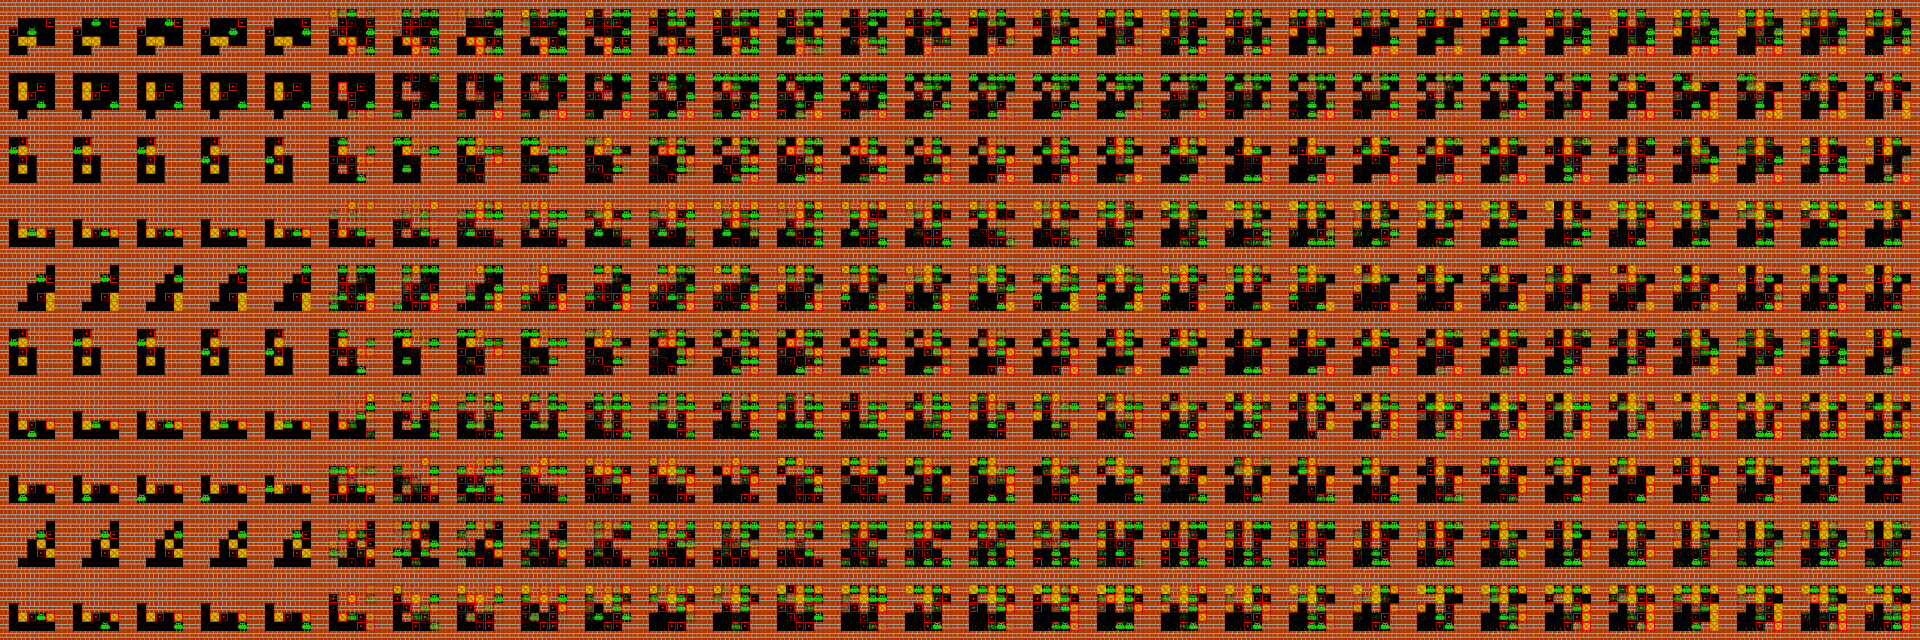
\includegraphics[width=1\textwidth,keepaspectratio]{figures/PlaNet/Sokoban_memory.png}
\caption[Qualitative result of the PlaNet model training in Sokoban]{Qualitative result of the model training in Sokoban. Each row depicts the model rollout in one episode. The first five columns include original consecutive observations from the evaluation dataset from which the rollouts start. The model hidden state was initialized on these transitions. Each subsequent reconstruction was obtained by first predicting the next latent state by the model and then decoding it using the decoder.}
\label{Fig.PlaNet_Sokoban_openloop}
\end{figure}

\subsection{PlaNet for Atari}

In this section experiments that lead to first successful case are described. The next section will focus on tuning this method to yield high scores, comparable to model-free methods, with the smallest amount of data possible.

\subsubsection{Train unchanged PlaNet in the Boxing environment}

It did not start to work out of the box of course. Fig.~\ref{Fig.PlaNet_Boxing_original} shows that future predictions turn into a blurry blob, where it is not possible to distinguish one player from another.

\begin{figure}[H]
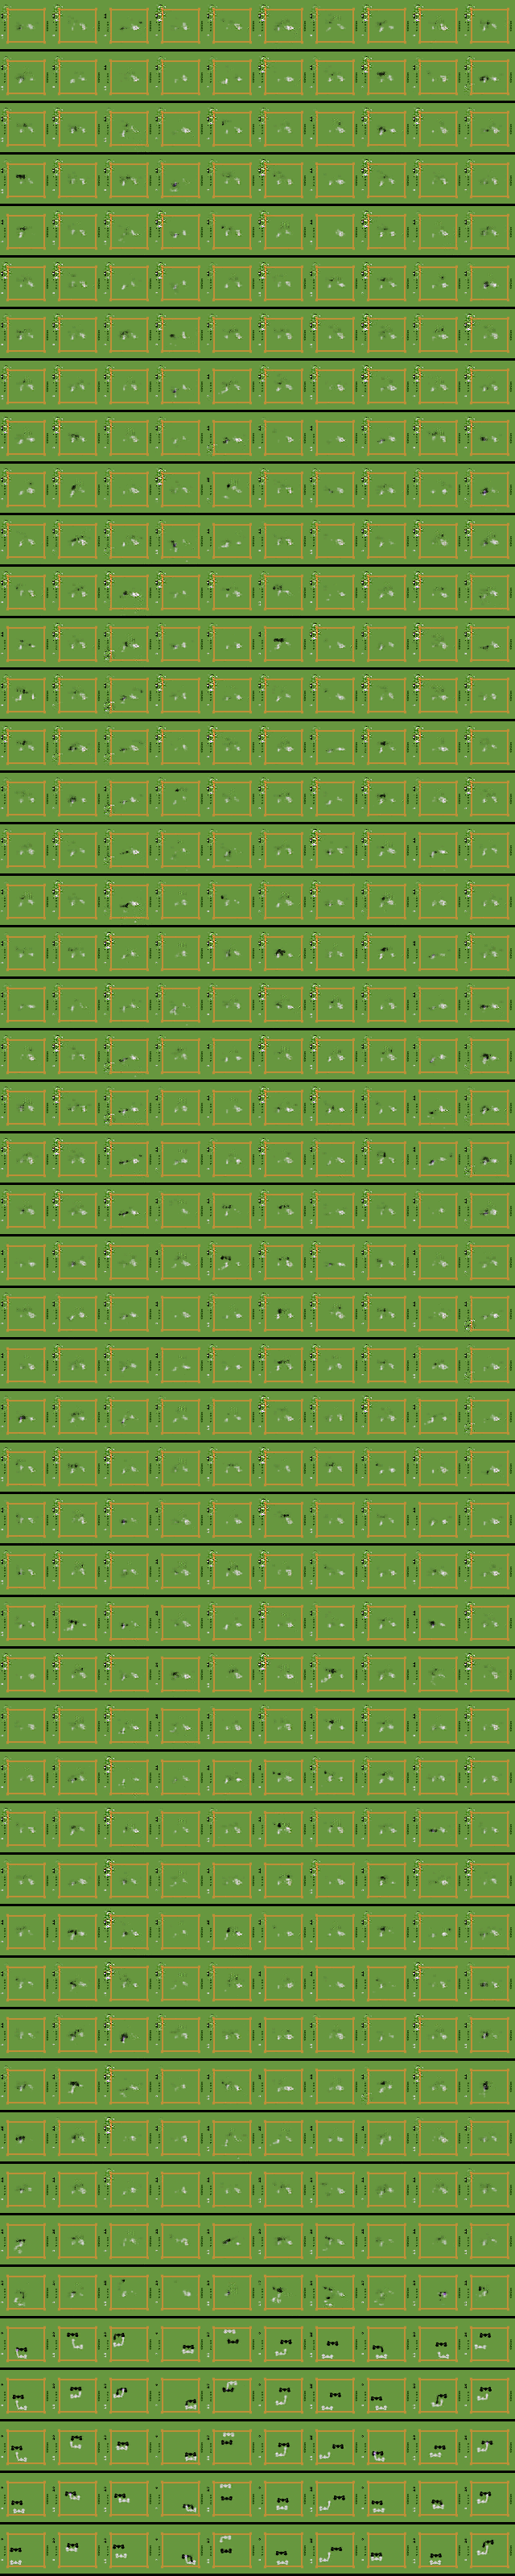
\includegraphics[width=1\textwidth,keepaspectratio]{figures/PlaNet/Boxing_memory_original.png}
\caption[Qualitative result of the original PlaNet model training in Boxing]{Qualitative result of the model training in Boxing. Each row depicts the model rollout in one episode. The first five columns include original consecutive observations from the evaluation dataset from which the rollouts start. The model hidden state was initialized on these transitions. Each subsequent reconstruction was obtained by first predicting the next latent state by the model and then decoding it using the decoder.}
\label{Fig.PlaNet_Boxing_original}
\end{figure}

By default a decoder variance of 1 is used, which means the model explains a lot of variation in the image as random noise. While this leads to more robust representations, it also leads to more blurry images. If the changes in consecutive frames are minor, then the posterior collapses because the model explains everything as observations noise. There are two possible solutions to this issue: one is to increase an action repeat and the other is to try to reduce the decoder variance. These are examined next.

\subsubsection{Train PlaNet in the Boxing environment with the increased action repeat}

The action repeat will result in a bigger difference between consecutive frames and thus more signal for the model to learn from, that cannot be easily modeled as noise. In practice though, it did not help and even made the agent play worse then a random agent. The random agent is taking moves at random.

\subsubsection{Train PlaNet in the Boxing environment with the lowered decoder variance}

The predictions are more blurry with a higher variance because the decoder generate more observations that differ slightly from the same latent code. This leads to the posterior explaining more similar observations with the same code. If consecutive frames are very similar, then the posterior collapses and explain them with one code. By lowering the variance it becomes more sensitive to small changes in observations. \editnote{TODO: Proofread this explanation once more and/or ask Danijar if it is right.}

Lowering the decoder variance is equivalent to lowering a KL divergence scale in the PlaNet loss. It can be seen by writing the ELBO for a Gaussian decoder in the standard form $E_q(z)[lnp(x|z)]-KL[q(z) || p(z)]$. The log-likelihood terms is $lnp(x|z) = -0.5(x-f(z))/\sigma^2-lnZ$. Multiplying the ELBO by $\sigma^2$ removes it from the log-probability term and puts it in front of the KL term as in beta-VAE \cite{Algo.betaVAE}. The objectives have different values because of the Gaussian normalizer Z but they share the same gradient since the normalizer is a constant.
Other reason that lowering the divergence scale can help with collapsing posterior is that it allows the model to absorb more information from its observations by loosening the information bottleneck.

On the other hand it is recommended to keep the divergence scale as high as possible while still allowing for good performance. For example, when the divergence scale is set to zero it could learn to become a deterministic autoencoder which reconstruct observations well but is less likely to generalize to state in latent space that the decoder hasn't seen during training.

Random search resulted in the best divergence scale being around 0.03. It was tuned jointly with a free nats parameter which is described in the next section.
\editnote{QUESTION: I should add diagram with random search results, but how to do this if those are evaluated with a researcher eye?}
\editnote{TODO: You should better describe this random search experiment. What parameters where tuned, which turned out to be the most important, for how long and how much runs you were running etc.}

\subsubsection{Train PlaNet in the Boxing environment with increased free nats}

Free nats technique is often used for static Variational Autoencoders. The model is allowed to use given amount of nats without KL penalty in variational objective. It helps the model focus on smaller details which do not contribute much to improving the reconstruction loss. Intuitively to this threshold of KL divergence (between a prior and a posterior) reconstruction loss is favoured. In case of Boxing, it helped to model boxers moves and actions more accurately. The best free nats turned out to be 12. Fig.~\ref{Fig.PlaNet_Boxing_lower_divergence_scale} shows final result.

\begin{figure}[H]
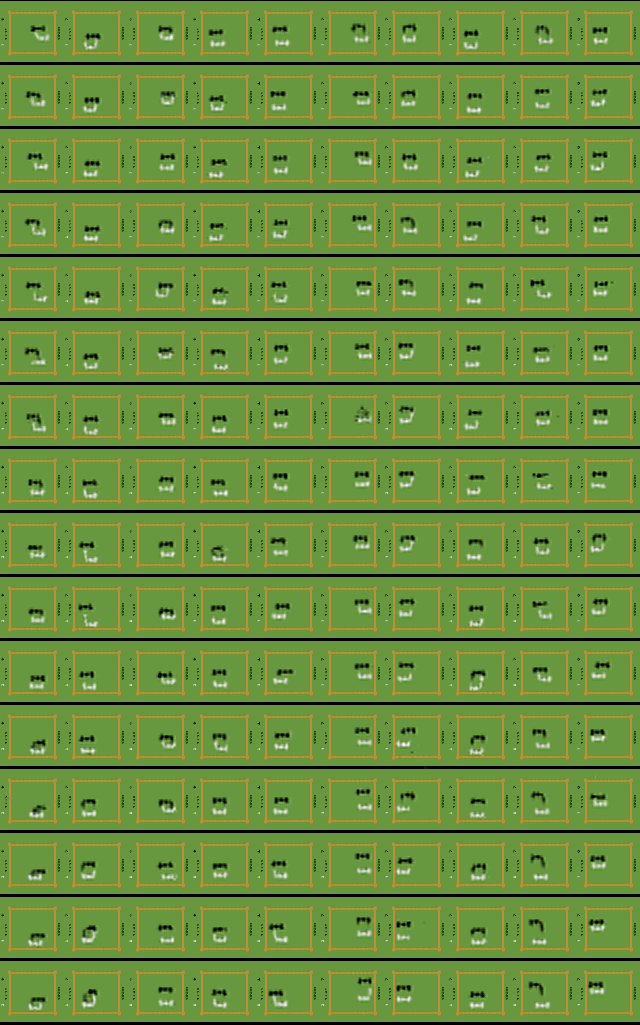
\includegraphics[width=1\textwidth,keepaspectratio]{figures/PlaNet/Boxing_memory_sharp.png}
\caption[Qualitative result of the PlaNet model training with a lower divergence scale in Boxing]{Qualitative result of the model training in Boxing. Each row depicts the model rollout in one episode. The first five columns include original consecutive observations from the evaluation dataset from which the rollouts start. The model hidden state was initialized on these transitions. Each subsequent reconstruction was obtained by first predicting the next latent state by the model and then decoding it using the decoder.}
\label{Fig.PlaNet_Boxing_lower_divergence_scale}
\end{figure}

It achieved final score around 30. \editnote{TODO: Download .csv with results from five Boxing training and plot nice curve.}

\subsubsection{Train tuned PlaNet in the Freeway environment}

The same random search procedure was applied to the Freeway environment described earlier. Fig.~\ref{Fig.PlaNet_Freeway_lower_divergence_scale} shows final result.

\begin{figure}[H]
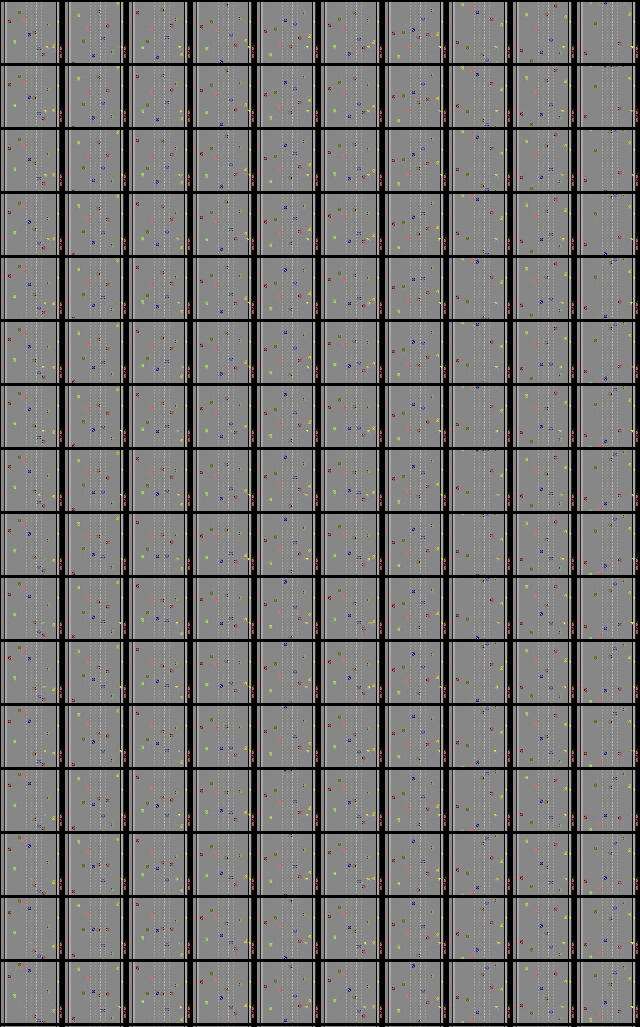
\includegraphics[width=1\textwidth,keepaspectratio]{figures/PlaNet/Freeway_memory_sharp.png}
\caption[Qualitative result of the PlaNet model training with a lower divergence scale in Freeway]{Qualitative result of the model training in Freeway. Each row depicts the model rollout in one episode. The first five columns include original consecutive observations from the evaluation dataset from which the rollouts start. The model hidden state was initialized on these transitions. Each subsequent reconstruction was obtained by first predicting the next latent state by the model and then decoding it using the decoder.}
\label{Fig.PlaNet_Freeway_lower_divergence_scale}
\end{figure}

Despite really good future observations prediction the agent failed to solve the task. \editnote{TODO: In benchmark description you should write what you consider as solved task in each environment.} Possibly planner horizon is to short to cover a plan which ends with positive reward on the other side of the road \editnote{TODO: In nomenclature or somewhere else you should clearly describe what is ``a plan''.}. This is explored in the next experiment.

\subsubsection{Train tuned PlaNet in the Freeway environment with a longer planning horizon}

\editnote{NOTE: This is the last experiment in progress, but it does not seem promising.}
